% !TEX program = lualatex
% !BIB program = biber
%\documentclass[oneside,paper=15cm:22cm,DIV=calc,pagesize]{scrbook}
% \documentclass[headinclude,12pt,DIV=12]{scrartcl}
% \usepackage{classicthesis}


\documentclass[letterpaper,12pt,oneside]{article}
\usepackage{booktabs}

\usepackage[left=1.5in,right=1.5in,top=1in,bottom=1in]{geometry}
\usepackage{graphicx}
\usepackage{subcaption}
\usepackage[binary-units=true]{siunitx}
\usepackage{float}
\usepackage{pgfplots}
\usepackage{listings}
\lstset{frame=tb,
basicstyle=\ttfamily,
language=Lisp}

\pgfplotsset{compat=1.14}

\tolerance=1000

\newcommand\mytodo[1]{[[\textcolor{red}{#1}]]}

\usepackage{microtype}
%\microtypesetup{protrusion=false,expansion=true,auto=true,tracking=true}
\hyphenation{block-chain}
\hyphenation{block-chains}
\hyphenation{Byz-an-tine}
\hyphenation{vir-tual-chain vir-tual-chains}
\hyphenation{crypto-curren-cy}


\usepackage{fontspec}
\setmainfont[BoldFont={* Semibold}]{Linux Libertine O}
%\linespread{1.1}
\setmonofont[Scale=MatchLowercase]{DejaVu Sans Mono}
\setsansfont[Scale=0.95]{Inter}
\usepackage{selnolig}
\nolig{Th}{T|h} % suppress "Th" ligature globally

%\usepackage{cochineal}

%\usepackage{libertine}

%\usepackage[sc]{mathpazo}
%\linespread{1.05}
%\usepackage{eulervm}

\graphicspath{{assets/}}

\usepackage{hyperref}
\hypersetup{
    colorlinks,
    citecolor=black,
    filecolor=black,
    linkcolor=black,
    urlcolor=black
}

% BibTeX
\usepackage[backend=biber]{biblatex}
%\renewbibmacro{in:}{}
\addbibresource{whitepaper.bib}

\begin{document}
\raggedbottom
\title{Synkletos: Themelio's collusion-resistant consensus mechanism}
\author{Themelio Labs}
\date{Version 1.0}
\maketitle

%\begin{abstract}

%\end{abstract}

\tableofcontents


\section{Introduction}

In the main Themelio whitepaper, we've described Themelio as if it were a magic oracle that always correctly maintains the world state and applies updates to it every block. In the real world, though, we require a \emph{consensus} procedure to ensure both \emph{consistency} --- all Themelio users observe the same world state $\sigma$ at every block height --- and \emph{validity} --- $\sigma$ can only change through valid transactions. In fact, consensus is what drives the two unique properties of blockchains we identified, endogenous trust and logical centralization. All security properties of blockchains are ultimately anchored in the design of the consensus mechanism.

Unfortunately, consensus is also a major source of instability and complexity in blockchains. Contentious blockchain governance problems are often tied to consensus-related issues such as decentralization (for example, the controversy surrounding Bitcoin block sizes), and attacks on existing blockchains, such as the 51\% attack on Namecoin, selfish mining attacks on Bitcoin, etc, focus on exploiting problems in consensus.

Blockchain consensus also differs with consensus in other distributed systems in how it must rigorously model trust within a game-theoretical model, rather than simply making assumptions about fault tolerance. To truly achieve incentive-compatible endogenous trust, we cannot rely on the typical approach of considering ideal ``honest'' behavior and then positing an ``adversary'' with certain powers. Yet cryptoeconomic mechanism design is still a young field full of uncertainties --- game-theoretical models often give results different from actual empirical observations --- and creating a consensus mechanism that is incentive-compatible under a wide variety of real-world conditions has proven to be pernicuously difficult. Nevertheless, we believe that we must abandon an ad-hoc approach to cryptoeconomic design --- that is, designing a consensus mechanism either heuristically or under simplified ``distributed systems'' security models, while analyzing the economics and incentives later, if at all.

Themelio takes a unique, ``economics-first'' approach to designing consensus and related cryptoeconomic mechanisms. We start by introducing a very pessimistic model: a blockchain totally controlled by one rational profit-maximizing entity. We consider what sort of blockchain rules would such a centralized business enforce, in the absence of external attackers. Perhaps surprisingly, we find that a rational monopoly would in fact behave in a trustworthy manner --- the problem with centralized systems is actually ``irrationality'', or rather hard-to-model utility functions.

Finally, we construct Themelio's decentralized consensus mechanism.
We show that a variant of proof-of-stake with a few critical departures from existing designs elegantly incentivzes a large, permissionless group of stakeholders to simulate this ideal rational entity as a whole, regardless of whether they coordinate their actions or not. This approach ensures that not only will consensus produce the desired results in a conventional ``non-coordinating majority'' world, Themelio's mechanism is actually \emph{collusion-proof}: a rational colluding majority will simply act the same way as our desired rational monopoly! Thus, Themelio avoids the pervasive yet fragile reliance on coordination costs to protect blockchain security.

\section{Goals and premises}

\subsection{The problem of coordination}

A commonly referred-to concept in blockchains is \textbf{coordination}. More specifically, we often see \emph{uncoordinated majority} assumptions, where the security of a blockchain relies on assuming that no more than some small fraction (usually between 25\% and 50\%) of consensus participants can coordinate their actions, and that participants are rational. For example, in Bitcoin we assume that no more than 50\% of the mining power can collude, or otherwise double-spending and similar attacks become profitable to the miner cartel.

Intuitively, this assumption seems very attractive. Coordination seems difficult in a permissionless blockchain: getting a majority of pseudonymous participants to agree to do something bad appears to be a costly ``cat herding'' exercise. Furthermore, collusion of a majority appears to be a scenario where the blockchain has already failed --- after all, decentralization is a central pillar of the entire appeal of blockchains.

Unfortunately, we believe that this entire paradigm is problematic. This is because ``coordination'' is a very slippery concept. For one, to even become consensus participants, users must in a broad sense coordinate to know about a blockchain, run compatible software, etc. Already, reality contradicts a theory of narrowly self-interested parties with no knowledge of or ability to contract with each other. Moreover, consensus participants in existing blockchains clearly coordinate in many ways not anticipated by the protocol. Ethereum miners, for example, almost unanimously vote for the same block size limit, while changing their votes in unison. These changes typically happen through out-of-band initiatives in forums and such.

So what prevents consensus participants from coordinating for ``evil'', if they routinely coordinate anyway? Indeed, some blockchains have fallen victim to protocol-violating collusion, such as when EOS's consensus participants decided to collude in censoring a set of accounts. It's not at all clear what game-theoretical incentives protect other blockchains from similar attacks.

We conclude that although very commonly used in blockchain design, uncoordination assumptions do not reflect reality and should not be used in Themelio. Instead, we start with a model that assumes the opposite --- a perfectly coordinated monopoly --- and then use cryptoeconomic incentives to simulate this model.

\subsection{A ``despotic'' blockchain}

Let's consider a ``blockchain'' operated by a single, profit-maximizing entity with control over the entire consensus. This entity is essentially a centralized business offering to add transactions to the blockchain for a price. What would be a rational course of action for this ``blockchain despot''? We show that such a despot would, in fact, behave in a reasonably ideal manner.

A seemingly obvious objection would be that the despot would greatly abuse the users of the blockchain, through double-spending, censorship, and similar attacks. Isn't the whole point of decentralization to avoid monopolies exploiting their customers? However, a \emph{perfectly rational} blockchain operator, constrained to offer blockchain services rather than simply choose a different line of business, would not choose such a course of action. The blockchain operator would like to establish a reputation to follow protocol rules correctly, or otherwise its customers will not continue using the blockchain and its only source of revenue disappears.

More generally, we would expect the following two behaviors to emerge:

\begin{itemize}
    \item The despot offers to include each transaction in the blockchain for a \textbf{revenue-maximizing fee}. This is the fee level at which further increases in fees would decrease revenue due to decreasing demand, and can be modeled using standard microeconomic monopoly models.
    \item The \textbf{minimum bribe} needed for the despot to engage in ``destructive'' behavior (such as disobeying the blockchain protocol) is the present value of the future lost fees of such behavior. This bribe need not be a literal bribe, but rather any sort of external payoff from disobeying the protocol. For example, if the operator also controls competing systems such as traditional payment networks, it might be in its interest to ``irrationally'' destroy the blockchain even without third-party influence.
\end{itemize}

Let's now show that first, the revenue-maximizing fee will not be extortionately high, and second, the minimum bribe will be a large fraction of the entire economic value generated by the protocol. This ensures that the ``average'' despot would be very trustworthy indeed.

\subsubsection{Revenue-maximizing fees}

The rational behavior of a revenue-maximizing monopoly is an elementary subject in microeconomics. The price that maximizes revenue for a monopoly depends on \emph{demand elasticity} --- the ratio $- \frac{dQ}{dP}$ between a small change $dP$ in price and a corresponding change $dQ$ in quantity demanded. For example, a good with a demand elasticity of $1$ will have demand increase by $1\%$ for every increase in supply by $1\%$. Generally, demand elasticity varies for the same good at different prices, increasing as price increases. To maximize revenue, a monopoly will charge at the price that gives a demand elasticity of $1$, where any increase in price will decrease quantity enough to reduce total revenue.

Unfortunately, studies of demand elasticity in blockchains are few and far between. In fact, to our best knowledge the only discussion of demand elasticity in blockchains is a forum post by Vitalik Buterin \cite{elasticity}. It examines a few ``natural experiments'' where the throughput of Bitcoin and Ethereum were reduced due to unexpected network conditions, coming to the conclusion that the demand elasticity of the Bitcoin fee market is between $0.4$ and $0.7$, while that of the Ethereum fee market is between $1$ and $2$.

Even from a ballpark estimate like this, we already see that the fees that a blockchain despot would charge cannot be far from those charged by existing blockchain protocols. In fact, though Buterin implies that the different elasticities are due to the different applications of the two blockchains, we think that a better explanation is simply that Bitcoin's low block size limit forces it to operate at a point in the demand curve with low elasticity, while Ethereum allows miners to vote on the gas limit to maximize revenue. A rational despot would certainly charge significantly lower fees, and produce more revenue, than Bitcoin does on average, and perhaps would charge similar fees to that of Ethereum.

%\textbf{TODO: large-scale curve-fitting of Bitcoin data? Is that even possible considering the block limit?}

\subsubsection{The price of bribing a despot}

We've established that a hypothetical despot would receive roughly the same level of fee revenue as Bitcoin and Ethereum do each year --- $1$-$3\%$ of the yearly on-chain economic activity $Y$. What would be the cost of bribing this despot to destroy the blockchain? This can be easily answered by calculating the present value of future fee revenue, which the despot must give up as a result of destroying the blockchain. This would range from $0.2Y$ assuming a high discount rate of $5\%$ and low revenue of $0.01Y$, to as much as $3Y$ with a discount rate of $1\%$ and an annual revenue of $0.03Y$.

To put this in perspective, for Bitcoin $Y \approx 300000 \mathrm{BTC}$, or around 2 billion US dollars. Even a low-end estimate of $0.2Y$ would exceed the cost of a 51\% attack on Bitcoin by many orders of magnitude. Thus, we see that \emph{assuming the despot is rational}, bribing him to damage his own cash cow would be much harder than attacking current blockchains.

\subsection{Decentralizing the despot}

Now that we've shown that a centralized blockchain operator would, rationally, behave quite ideally. Why do we even bother with decentralization? The answer is that there are two assumptions in the analysis that we can't rely on in the real world --- that the despot is perfectly rational, and that it has a utility function valuing only monetary revenue. In the real world, centralized businesses often make irrational, non-profit-maximizing decisions, and they are subject to a wide variety of utility-function-distorting pressures such as government regulation and public opinion. Thus, we simply cannot trust that a centralized operator would in fact behave like our hypothetical blockchain despot.

However, we believe that our ideal despot is indeed a good model for a \emph{coordinated coalition} of decentralized parties. Decentralization ensures that the utility function of the group as a whole will be that of an ``average'' despot, which will not have idiosyncratic factors that prevent our analysis from working. This gives us Themelio's main  mechanism design goal --- creating a mechanism that \emph{simulates a rational blockchain despot} by coordinating many parties, some of which might not be able to coordinate without help.

This may seem to be a rather weird framework. After all, a blockchain despot will rationally make quite a few suboptimal choices, such as demanding fees higher than those that will maximize social utility. The reason why we choose this approach are twofold:

\begin{itemize}
    \item \emph{Robustness against out-of-band collusion}: Essentially, Themelio's protocol mechanisms are designed to coordinate participants to act the way they would if they could perfectly collude out of band. Thus, we eliminate the risk of cartels breaking protocol guarantees.
    \item \emph{Creates a single Nash equilibrium}: Even if we harden a traditional blockchain protocol based on a non-coordination equilibrium against malicious cartels, it would be difficult to avoid different behavior in a non-coordinated and coordinated world (say, significantly different fee levels). Such a blockchain would have multiple stable equilibria, causing uncertainty as to which ``world'' applications will operate under in the future and turmoil during transitions between equilibria. Themelio's approach, on the other hand, ensures stable behavior even as coalitions potentially form and disband.
\end{itemize}

We describe how we construct this decentralized despot in two parts. First, we outline Themelio's proof of stake mechanism called Synkletos\footnote{From Greek for ``senate'', a reference to the Byzantine Senate}, which uses a unique dual-token system to incentivize blockchain-despot-like behavior and mitigates the well-known ``weak subjectivity'' problem of proof-of-stake systems by dividing time into ``stake epochs''. We then look at Themelio's novel fee and reward system that supports the incentives of Synkletos through a mechanism that safely funds almost all protocol rewards through user fees.

\section{Synkletos: consensus in Themelio}

Now let's look at Synkletos, Themelio's proof-of-stake consensus mechanism. We first discuss Synkletos' tripartite division of users into stakeholders, auditors, and clients. We then examine the roles each of these classes play in maintaining Themelio's decentralized ``despot simulation''.

\subsection{Three kinds of nodes}

Participants in Themelio are divided into three categories by their roles:

\begin{itemize}
    \item \textbf{Stakeholder nodes} record transactions into new blocks and confirm them using a Byzantine fault-tolerant consensus algorithm between themselves. They communicate with each other through a broadcast protocol which other nodes in the network never participate in. Anybody can become a stakeholder by locking up a significant amount of cryptoasset as collateral, similar to other PoS systems like Casper. Stakeholders correspond to miners or validators in other systems.
    \item \textbf{Auditor nodes} download newly created blocks from the stakeholders and gossip them between themselves while mirroring the entire world state. Anybody can join the network as a auditor by simply running a piece of software. Auditors verify new blocks decided by the stakeholders and check that the stakeholders never equivocate on the content of a given block height. Auditors roughly correspond to full nodes in other systems, although they have a more important role in Themelio's security.
    \item \textbf{Client nodes} are lightweight participants that query the network of auditors to access specific information in the blockchain, yet do not trust any particular auditor.
\end{itemize}

Essentially, the stakeholders create blocks through a proof-of-stake consensus, but auditors check their results, and everything can be queried by clients. Let's now see how this actually works.

\subsection{Stakeholders: the oligarchy}

Themelio uses a variation on a classic technique known as bonded proof of stake, used in systems like Tendermint and Casper. We keep track of a special secondary currency on the blockchain known as the \textbf{sym}, Greek for ``share'' in the financial sense. Syms are traded freely alongside mels, the main cryptocurrency of Themelio, with a relatively unchanging supply. They can be thought of as equity ``shares'' in the distributed blockchain despot, sharing both control and revenue.

In order to become a stakeholder, one \textbf{stakes} at least 1,000 syms, locking them up for a fixed period of time (at least 500,000 blocks, or approximately 6 months) as a performance bond. During that period of time, the stakeholder obtains voting rights in a  consensus algorithm in proportion to the amount of syms staked. Furthermore, the stakeholder staking $x$\% of all staked syms receives revenue in proportion to $x$\% of all economic value provided by Themelio. This ensures that the value of a sym $v$ is proportional to the total economic value of Themelio $Y$ divided by the number of staked syms $S$: $v \propto Y/S$. We will discuss how this is accomplished in \ref{sec:fees}.

\subsubsection{Byzantine fault-tolerant consensus}

The stakeholders come to agreement on each block through a partially synchronous Byzantine fault-tolerant (BFT) consensus algorithm. Formally, we abstract this as a protocol $(\sigma', \pi_{\sigma'}, B) := \mathsf{BFT}(\sigma, T^*_\mathrm{tentative})$ deciding the next block from the current state, run at every stakeholder node, where
\begin{itemize}
    \item $\sigma$ is the current world state
    \item $T^{*}_\mathrm{tentative}$ is a tentative proposal of transactions to include in the next block, which may not be consistent across all stakeholders.
    \item $B$ is the newly produced block, consistent across all honest stakeholders.
    \item $\sigma'=\Omega(B, \Upsilon^*(\sigma, T^*_{\mathrm{final}}))$ is the new block state, consistent across all honest stakeholders, where $T^*_{\mathrm{final}}$ is the decided set of transactions in the new block.
    \item $\pi_{\sigma'}$ is a \emph{consensus proof} consisting of a list of cryptographic signatures by stakeholders, each signing $\mathsf{B2H}(\sigma')$.
\end{itemize}

$\mathsf{BFT}$ also has the following three properties:
\begin{itemize}
    \item \emph{Accountable safety}: as long as at least $2/3$ of the syms staked by the stakeholders belong to protocol-following stakeholders (``there is a quorum''), all honest stakeholders agree on the same $\sigma'$, and $\sigma'$ must be the result of applying a valid block-level state transition to $\sigma$. Furthermore, every protocol-following stakeholder will only sign one proposal for $\sigma'$, so two valid consensus proofs of the same block height will never occur if there is a quorum.
    \item \emph{Liveness}: as long as there is a quorum, the protocol will make progress.
    \item \emph{Fairness}: each stakeholder's proposal is accepted roughly in proportion to its share of all staked syms.
\end{itemize}

In the current implementation of Themelio, we use HotStuff as an implementation of $\mathsf{BFT}$, but the actual choice is not really important. This is because the consensus proof $\pi_\sigma'$ encapsulates the result of the consensus algorithm, and the rest of the details are invisible from the rest of the network. In fact, we don't consider the BFT consensus algorithm itself to be part of the ``consensus-critical'' core that must stay stable over time! Any changes must be backwards-compatible, but fundamentally as long as compatible consensus proofs are generated, stakeholders are free to switch to different BFT consensus algorithms.

\subsubsection{Why proof-of-stake?}

Why did we choose PoS over other consensus algorithms, such as the venerable proof of work (PoW) of Bitcoin, or the proof of authority (PoA) found in consortium and private chains? There are both general reasons that apply to all proof-of-stake systems, and also a reason more specific to how Themelio uses proof of stake. The Ethereum Proof-of-Stake FAQ \cite{buterin2019pos} give a strong defense of PoS; some properties of PoS in general we consider especially important for Themelio include:


\begin{itemize}
    \item \textbf{Higher security margin}: Attacking a PoS blockchain directly requires expending an vast amount of resources to buy up stake. This is equivalent to around 1/3 of the total value of staking coins (a proxy of the economic value of the blockchain system). Thus, as usage increases, PoS  security will proportionately strengthen until it becomes practically invulnerable to attacks on the consensus protocol. Proof-of-work blockchains like Bitcoin, however, can be subverted quite cheaply. Attacks reverting a full hour of Bitcoin transactions cost less than \$1,000,000 \cite{crypto51}, pocket change compared to the almost \$100 billion Bitcoin market capitalization. Finally, proof of authority, which is not a decentralized solution, is very fragile to centralized attack vectors such as hacking or government regulation.
    \item \textbf{Immediate finality}: PoS allows easy, secure finality using asynchronous Byzantine fault-tolerant consensus protocols. This means that as long as we have a quorum, a block that is successfully appended to the blockchain will never be reverted. This eliminates the unpredictable behavior found in ``chain-based'' consensus protocols like proof of work, such as forks and block reorganizations. More importantly, it eliminates the implicit trust in network synchronicity found in ``longest-chain'' style consensus algorithms, preventing eclipse and similar attacks.
    \item \textbf{Stronger incentive compatibility}: As we will see shortly, staked bonds allow us to punish misbehaving stakeholders by deleting their stake. In other blockchains, misbehaving miners only lose potential rewards or reputation. As the Ethereum FAQs put it, ``in PoW, we are working directly with the laws of physics. In PoS, we are able to design the protocol in such a way that it has the precise properties that we want - in short, we can optimize the laws of physics in our favor.''
\end{itemize}

The most important reason why we use proof of stake with a special staking token, however, is that it \emph{distributes the utility function of a hypothetical despot} to all participants. Intuitively, this is because the stakeholders as a whole receive the same consequences of their collective actions as a despot, while syms, being valued as fractions of the revenue of the stakeholder collective due to $\mathsf{BFT}$'s fairness property, would depreciate and appreciate to replicate these consequences in proportion to the number of syms someone owns. This relies crucially on the fact that the sym is an ``equity'' share; a single proof-of-stake system using a currency-like coin, such as that proposed for Ethereum, would not have such an elegant incentive structure.

A more complete account of how the incentives work, though, would have to wait to \ref{sec:fees}.

\subsubsection{Performance vs decentralization}

Scalable blockchains with immediate finality need a way to limit the number of consensus participants. This is because Byzantine fault-tolerant consensus algorithms have rapidly increasing overhead with increasing participants. To achieve our key design goal of scalability and performance and avoid DoS attacks, we cannot simply allow a limitless number of stakeholders.

Themelio's way of restricting the number of stakeholders is through the minimum requirement of 1,000 syms staked per validator. Essentially, we limit entry into the oligarchy of stakeholders to only the richest sym holders. Since sym supply follows a fixed schedule, this places a hard limit of a few hundred new validators a year, so that growth in overhead won't outpace growth in computational capacity.

%\textbf{TODO: hardcoding this might not be the best approach. Is there a good way to let the market decide without running into collective action problems?}

Although this is a very simple mechanism of restricting the number of consensus participants, it does not seem to be popular among existing proof-of-stake variants. We think this is most likely because a large minimum stake is politically unappealing. After all, it ``disenfranchises'' the vast majority of potential stakeholders and institutes a ``plutocracy''! Unfortunately, other approaches that superficially sound more decentralized tend to have crippling problems. Ironically, they end up a lot more vulnerable to centralized threats.

For example, a common method of deriving a small amount of participants from a large body of coinholders is \textit{delegated proof of stake} (DPoS). In DPoS, coinholders vote for people with voting power proportional to their coin ownership, and only the few with the most votes become ``delegates'' and participate in consensus. EOS is a popular blockchain using DPoS.

Yet although DPoS gives a vote to all coinholders, it insulates coinholders from protocol incentives. Coinholders are not responsible for the actions of the delegates they vote for, while misbehaving delegates receive no punishment other than a loss of reputation. Thus, coinholders have no incentive to vote for ``good'' nodes, delegates have little incentive to behave correctly, and misbehavior is rampant. Unsurprisingly, all the problems of political governance in a representative democracy get imported. Elections involve massive advertising campaigns, vote-buying, and even nationalist agitation \cite{zhihu2019votebuy}, while delegates often behave as a centralized cartel, engaging in actions like censoring transactions \cite{eoscensor}.

\textit{Sortition} is another approach, used most notably in Algorand \cite{gilad2017algorand}. Periodically, a committee of participants is randomly selected from all coinholders --- each coinholder has a probability to win this ``lottery'' in proportion to the coins that they hold. The committee then participates in a consensus protocol to decide new blocks until the next lottery comes around.

Sortition eliminates most of the politics-like problems of DPoS, allowing protocol incentives like rewards and slashing to work fairly well. Unfortunately, severe problems remain. Randomly selecting participants trustlessly turns out to be a surprisingly hard cryptogrpahic problem --- a corrupt lottery can reliably elect malicious committees. Bribery attacks also become much easier, since instead of buying 1/3 of the coins, attackers can simply bribe the current committee, who has only a small fraction of the stake. Complex consensus protocols and advanced, non-quantum-resistant cryptographic techniques can reduce both challenges. But ``fancy'' mechanisms generally go against Themelio's philosophy of future-proof simplicity.

A point must be made that \textit{blockchain consensus is not analogous to political governance}. Themelio's ``plutocratic oligarchy'' of stakeholders certainly does not make for an effective way of electing a parliament. But for blockchains, it yields highly robust and decentralized security, because we don't pursue decentralization for its own sake. Instead, it is simply to average out individual interests to simulate a blockchain despot, implying that \emph{decentralization has rapidly diminishing returns}.

Thus, we do not believe that Themelio's ``plutocratic'' bonded proof of stake is any more vulnerable to centralized threats than PoS blockchains without minimum stake amounts. Even so, as we will immediately see, Themelio has a system of \textit{auditors} keeping stakeholders in check, ensuring that even a fully corrupted quorum of stakeholders cannot do much damage.

\subsection{Auditors: keeping stakeholders in check}

\subsubsection{Making failure catastrophic} \label{sec:nuke}

The second role in Themelio belongs to the \textbf{auditors}. Auditors are ``full nodes'' in usual terminology, replicating and validating the entire blockchain. They form a random \emph{gossip} network among themselves, similar to that used by Bitcoin full nodes. Through this gossip network, information about new blocks is disseminated. Gossip reduces load on the stakeholders and makes it difficult for malicious networks to censor the blockchain --- as long as some auditors can connect to the stakeholders and the auditors form a connected graph, new blocks will quickly be visible to every auditor.

The more important role of auditors, though, is to \textit{make consensus failure catastrophic}. This plays a crucial role in replicating the utility function of a blockchain despot to the oligarchy of stakeholders. Auditors utilize their position as relayers of new blocks to continually monitor for cryptographic evidence that the stakeholder consensus is corrupt. This is either a consensus proof $\pi_\sigma$ with an invalid state $\sigma$ (``invalid state''), or two consensus proofs $(\pi_{\sigma_1},\pi_{\sigma_2})$ where $\sigma_1.\mathsf{height} = \sigma_2.\mathsf{height}$ but $\sigma_1 \neq \sigma_2$ (``equivocation'').

Any auditor that sees a consensus nuke immediately broadcasts it to all auditors it knows in the gossip network. It then permanently activates a ``kill switch'' and refuses to operate normally. Thus, an attempt at forking or appending invalid transactions to the blockchain would destroy the entire network.

\subsubsection{Why consensus nukes?}

This objective seems a little strange. Why would we ever want our network to self-destruct?

The obvious answer is that if we no longer have a 2/3 supermajority of honest stake, the entire system is irrecoverable. More specifically, a well-known result \cite{dwork1988consensus} mathematically proves that consensus protocols running in a partially synchronous network model (that is, network delays are unknown but finite) cannot possibly tolerate more than 1/3 arbitrary faults. So we have to choose between a model where the network stays up, but malicious stakeholders can corrupt the state arbitrarily (rewriting history, giving themselves free money --- or shutting down the network), or one where the only thing a corrupted quorum can do is shut down the network. Clearly, the latter is preferable.

Much more importantly, consensus nuking changes the incentives of potential attackers by making breaking the consistency of the blockchain unprofitable for our hypothetical blockchain despot. Consider a blockchain where consensus-breaking attacks (like Bitcoin's 51\% attack) allow arbitrary state corruption. A malicious actor with control over consensus can extract huge profits simply through double-spending. With more complex higher-level applications relying on blockchain data, profit opportunities are even more numerous. Thus, if self-serving stakeholders rationally collude, they are greatly incentivized to attack the network and destroy its security guarantees.

If a successful attack can only result in the network stopping all work, an ``average'' profit-maximizing despot will not execute such an attack and destroy their future revenue stream. Instead, only attackers who benefit from destroying the network will participate, and even then, they must control a vast amount of syms to be able to launch a consensus-breaking attack.

Finally, a shutdown when a successful attack occurs forces Themelio users to manually coordinate an emergency ``hard fork'' out-of-band to restore the network. This would involve, at the very least, a redistribution of stakes away from the attacking parties and possibly protocol improvements to prevent future attacks. On the other hand, if the blockchain continues to operate even when stakeholders are corrupting the state, nothing forces users to coordinate a hard fork. It's conceivable that the malicious stakeholder cartel can create a climate of pressure for users to go along with the corrupted chain --- for example, the state corruption might be forced by legal regulation or presented as way of restoring stolen assets. Consensus nuking ensures that these scenarios are impossible.

\subsection{Clients: scalable consumers of endogenous trust}

Most users of a blockchain, Themelio not excepted, do not have nearly enough resources to process all transactions 24/7. Users that do not synchronize the whole blockchain state, known as thin clients, serve a vital role in any blockchain system. In other blockchains, though, thin clients come with both reduced security and mediocre performance. Bitcoin, for example, has thin clients who must persistently store a growing set of block headers and connect to at least one trusted full node.

In Themelio, thin clients (usually just called clients) are both thinner and safer than thin clients in other systems. Clients only synchronize a small piece of data, less than a kilobyte in size, a few times a year. Yet with this data, they can fully validate a large variety of information they can freely obtain from auditors. Even if a client only connects to bad auditors, it cannot be fooled into accepting invalid data. We accomplish this through two features: \textit{state commitments} in block headers and \textit{stake epochs}.

\subsubsection{State commitments}

As we've previously seen, at every block height $h$ Themelio cryptographically commits to its world state $\sigma_h$ through a block header. This allows us auditors to generate short proofs about the content of the current world state. More specifically, given any key $k$ and an SMT tree root (for example $\sigma_h.\mathtt{transactions}$), an auditor with access to the world state can generate either a proof that $k$ is bound to a specific value $v$, or that $k$ does not exist in the mapping. This proof is only of size $\Theta(\log n)$, where $n$ is the number of values in the SMT.

What this means is that given that it somehow obtains the latest block header from a trustworthy source, a thin client can easily check the status of coins and transactions by simply asking an untrusted auditor. This allows clients to trustlessly interact with Themelio's state in quite a complex manner. Note that although this process is reminescent of Bitcoin's SPV (simple payment verification) protocol \cite{nakamoto2008bitcoin}, a major difference exists in that Bitcoin does not commit to it world state in a way that allows easy proofs. Instead, Bitcoin only commits to the content of each block, allowing for proofs that a transaction was included in a block, but the actual status of coins in the world state can only be trustlessly determined by downloading all transactions and appling them to the genesis state. Thus, even very simple Bitcoin applications, such as wallets, cannot operate with truly endogenous trust and must rely on a trusted full node.

Of course, all this assumes that the client can in fact obtain the latest block header trustlessly. This is accomplished by the second pillar of Themelio's thin client system, stake epochs.

\subsubsection{Stake epochs} \label{ss:stakeepochs}

How are clients supposed to get the latest block header? In many blockchains, clients simply synchronize \emph{all} the block headers. Clients can then use the consensus proof embedded in each header to verify the next. In ``longest-chain'' proof-of-work blockchains such as Bitcoin, this consensus proof is simply a valid proof-of-work solution. In Themelio's case case, it would be the value $\pi_\sigma$ produced by $\mathsf{BFT}$.

Unfortunately, such a strategy would be prohibitively expensive in Themelio. $\pi_\sigma$ contains cryptographic signatures from at least 2/3 of the stakeholders --- this is at least 64 bytes (the size of an ed25519 signature) for every stakeholder, and would take up dozens of kilobytes. Combined with Themelio's 30-second block interval, the block header consensus proofs spanning a year would amount to more than 10 GB.

To fix this problem, Themelio divides blocks into \textit{epochs} lasting 500,000 blocks, or about half a year. Within each epoch, the list of shareholders and their respective voting weights stays the same. All stake-related transactions, such as staking and slashing, take effect \emph{only at the start of the next epoch}. When validating the $h$th consensus proof $\pi_{\sigma_h}$, we actually use the stake document $\sigma_{\lfloor (h-1)/500,000 \rfloor}.\mathtt{stakes}$ rather than the immediately preceding one.

Through this process, a client can quickly ``skip back'' until it reach a stake document it already knows. For example, to validate block header 1,100,000, we need the stake document embedded at height 999,999. But to validate the world state that height, we need the stake document at height 499,999, etc.

Thus, to synchronize with the clients simply have to catch up on all the new stake documents they missed --- a few dozen KB every 6 months. Afterwards, they can securely validate the latest block header, which then lets them query the content of the world state without trusting anyone. Such ultra-thin clients allows very good \emph{read scaling}: billions of small devices like smartphones can easily query the world state while keeping trust totally decentralized.

\section{Fees and incentives} \label{sec:fees}

In this section, we describe how Themelio's unique fee and incentive structure coordinates the behavior of a decentralized group of stakeholders to approximate that of a ``blockchain despot''. This is accomplished by a fee mechanism that incentivizes stakeholders to charge fees at the same level that a despot would charge, while backing the value of their stakes with these fees.

\subsection{Syms as equity shares}

Earlier, we mentioned that Themelio uses a special secondary currency, the \emph{sym}, in its proof of stake mechanism. We hand-waved it as having ``equity-like'' properties, but what exactly does that mean?

Consider the revenue-maximizing blockchain despot. Such a despot would charge fees as to maximize the economic value captured. Let's assume that Themelio's protocol can somehow charge fees exactly the way a despot would, and that these fees are distributed to stakeholders in proportion to their stake. For example, if there are only two stakeholders, Alice staking 10 syms and Bob staking 30 syms, and the despot-simulating protocol collects 100 mels of fees a day, Alice would be paid 25 mels/day while Bob would be paid 75 mels/day.

In such a model, staked mels are simply shares in the revenues of this simulated despot. Assuming that markets are efficient, then, the real value of each stakeholder's stake is proportional to that of the discounted future revenue of the stakeholders as a whole. This is crucial to our goal of having the stakeholders coordinate to simulate a single entity --- any action that would harm or benefit a despot would have proportionate harms or benefits to every single stakeholder.

For example, censoring transactions, an action that generally requires majority coordination, would certainly harm the long-term economic value of Themelio and thus the revenue stream of our hypothetical despot. Thus, a rational despot with no external incentives will not choose to censor transactions. In Themelio's actual world of disparate stakeholders, coordinating to censor transactions will similarly harm each and every stakeholder, and thus no rational stakeholder would have an incentive to participate in such a malicious act. Furthermore, an adversary wishing to bribe stakeholders to take value-harming actions will have to compensate each stakeholder for their expected loss of revenue --- a value equivalent in total to bribing a despot.

There are two remaining pieces in the puzzle:
\begin{itemize}
    \item First, \emph{how do we generate a stream of fees that simulates the income of a revenue-maximizing despot}? The solution is a fee and reward system very different from that of existing cryptocurrencies, which we will show incentivizes even uncoordinated stakeholders to coordinate in charging fees at the right level.
    \item Secondly, \emph{how to prevent failures due to discoordination}? Unlike most blockchain protocols that assume uncoordinated participants, Themelio assumes a world where stakeholders may rationally choose to coordinate their actions. Yet we must avoid prisoner's dilemma-type situations where uncoordinated rational choices produce outcomes divergent from that of a unified despot. This is done through two exceptional mechanisms in the incentive system --- slashing and nuking.
\end{itemize}


\subsection{Stable and incentive-compatible fees} {ss:stablefees}

As in Bitcoin and other public blockchains, each transaction in Themelio includes a transaction fee to compensate stakeholders and make flooding attacks costly. Most other blockchains let transaction senders voluntarily decide whatever fee they like; block creators then decide which transactions to include in the limited space within a block. This functions as a pretty fair and efficient first-price auction, since transactions with more fees relative to the burden they pose to the network get higher priority. Unfortunately, auction-based transaction fees paid to whoever included the transaction in a block have two significant problems:

\begin{itemize}
    \item \textbf{Volatile, unfriendly fees}. When blocks are filled, average fees will vary quite a lot as demand fluctuates. In practice, persistently full blocks is the norm, whether due to demand increase in protocols like Bitcoin where the block size cap is fixed, or due to block producers setting block limits according to demand as in Ethereum. Thus, fees for full blocks are extremely volatile in existing blockchains, often changing as much as 2x within one block interval. This makes for a very poor user experience.

          Furthermore, it's difficult to determine how much fees to bid in order to get transactions confirmed in a traditional fee market. Wallets need complicated algorithms to estimate the right amount of fee based on looking at unconfirmed transactions --- which thin clients can't even securely monitor. All this tends to greatly increase the friction of using the blockchain.
    \item \textbf{Coordinated and uncoordinated rationality sharply diverge}. Finally, a fee market based on a first-price auction has severe incentive problems. In the most well-known instance, if participants' have revenue largely derived from fees --- a requirement for Themelio's fee-backed syms to work --- pathological, protocol-violating behavior can result under a uncoordinated rationality assumption \cite{carlsten2016instability}. Other blockchains typically mitigate the worst of the problems by funding consensus participation primarily with monetary inflation, a choice Themelio cannot make.

          The real problem underlying the game-theoretical ``nastiness'' of first-price fee auctions, however is that even ideal uncoordinated rational behavior is very different from coordinated rational behavior. In particular, ignoring the pathological cases described in \cite{carlsten2016instability}, uncoordinated block creators normally want to include as many transactions as possible in their own blocks as long as they pay fees exceeding the cost to process them. This is in contrast to a ``despot-simulating'' coordinated cartel, which would want to reject some transactions that would be profitable on the margin in order to jack up the average fee level towards the revenue-maximizing point. As a rule of thumb, games where uncoordinated equilibria greatly differ from coordinated equilibria tend to be prone to pathological strategies --- and in any case, our design philosophy strongly favors collusion-proof incentive structures.
\end{itemize}

Thus, we abandon the traditional fee auction model in favor of a system inspired by EIP-1559 \cite{eip1559}. Every transaction pays a mel-denominated fee that has two components. A mandatory \textit{base fee} $\mathsf{BaseFee}(t) = \beta \cdot \mathsf{Weight}(t)$ for a transaction $t$ is calculated by multiplying by the \textit{base fee multiplier} $\beta$ and the \textit{weight} of a transaction, a metric that roughly measures its cost. Transaction senders can then add a \textit{tip} above and beyond the base fee.

Every time a new block is created, the stakeholder proposing the block can adjust the base fee multiplier by up to 1\% upwards or downwards --- the base fee multiplier then reflects the stake-weighted median of the stakeholders' preferences. Base fees are deposited into a special \textit{fee pool} regardless of who included the transaction into the blockchain; the stakeholder creating a block then withdraws a tiny fraction ($1/65536$) of the fee pool. The net effect is that the base fee of a transaction is distributed to all stakeholders regardless of who made the block that contains the transaction.

Tips, on the other hand, are simply paid to the block producer, like fees in traditional blockchains. We expect tips to be a small fraction of total fees, and they give an incentive for block producers to actually include transactions instead of freeloading on a fee pool replenished by other, more honest block producers.

\begin{figure}
    \centering 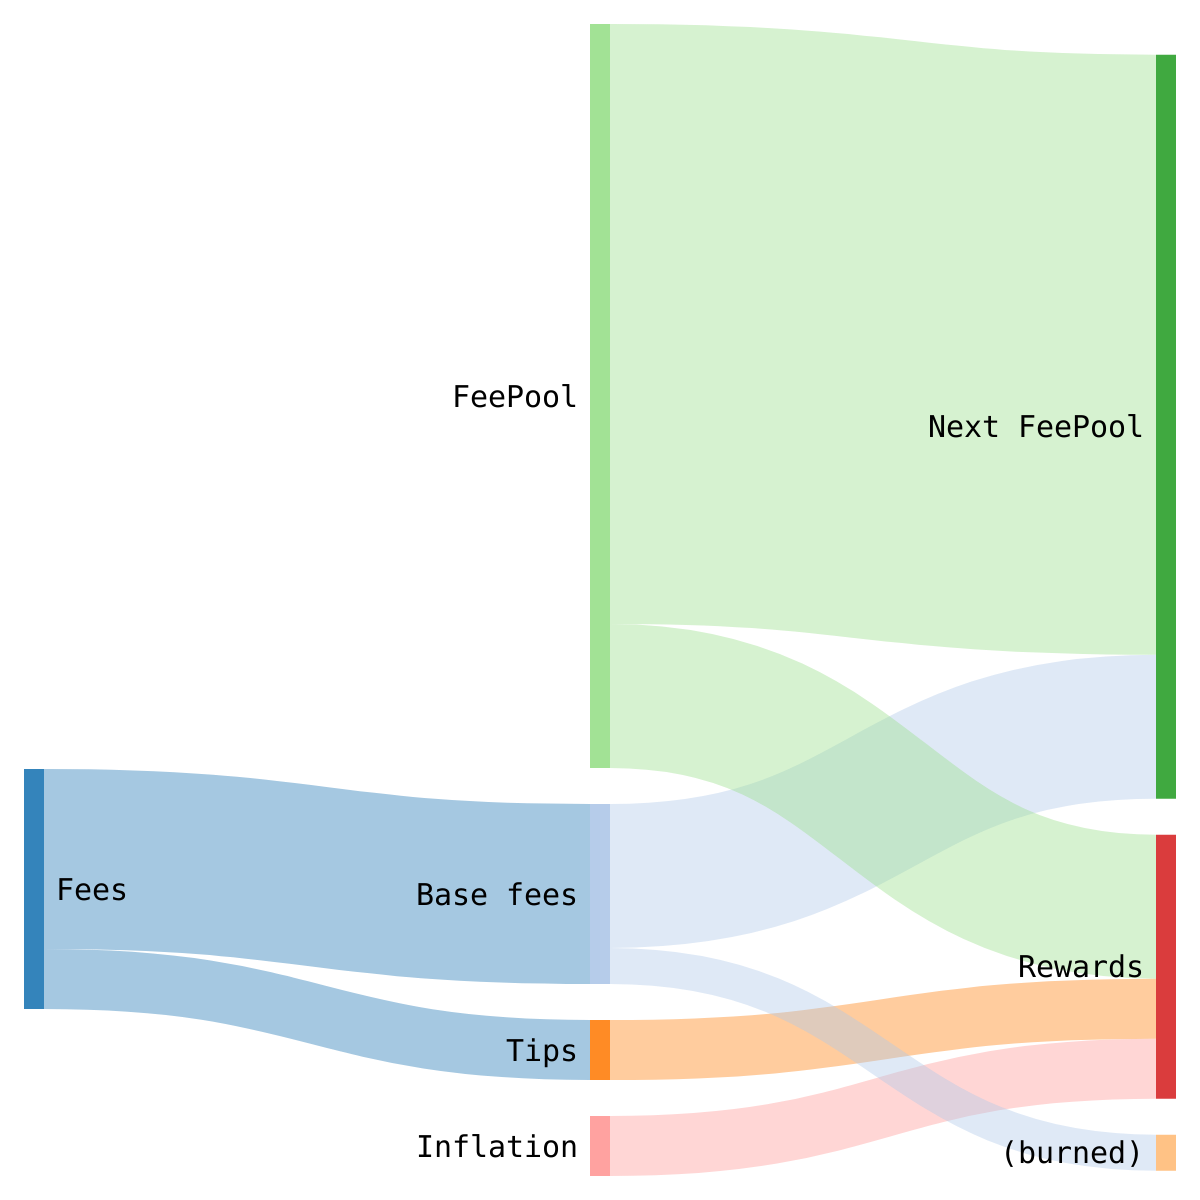
\includegraphics[width=0.5\linewidth]{fees.png}
    \caption{Per-block producer rewards (including sym inflation)}
    \label{fig:fees}
\end{figure}

Figure \ref{fig:fees} illustrates the flow of funds every time a new block is created.

Themelio's fee system fixes both fee unpredictability and incentive compatibility. It's comparatively easy to see why fees would be much more predictable --- base fees are charged at a publicly announced, slowly-changing value, and ``base fee + small tip'' will be a working strategy for clients in almost all situations.

Incentive compatibility is a little trickier. We assume that there is a single revenue-maximizing fee multiplier $\hat{\beta}$, where for a blockchain despot, charging a fee of $\beta \cdot \mathsf{Weight}(t)$ for each transaction $t$ is the revenue-maximizing strategy. Furthermore, we assume that given any two multipliers $\beta$ and $\beta'$ where $| \beta' - \hat{\beta} | < | \beta - \hat{\beta} |$, $\beta'$ generates more revenue in the long run than $\beta$. Informally, this just means that nudging a suboptimal price closer to $\hat{beta}$ would always be profitable for a despot.

Let's now analyze one specific situation --- one specific stakeholder assembling a block to propose as the next block in the blockchain. In a world of perfectly coordinated stakeholders, this stakeholder will of course nudge $\beta$ closer to $\hat{\beta}$ and include as many valid transactions as possible, in accordance to the strategy we assume is optimal for a despot. Furthermore valid transactions will be included even without tips, since setting the base fee signals the reservation price of the stakeholder cartel much better than refusing to accept transactions without the right tip. Let's now show that even when the stakeholder must make a decision without coordinating with others, he will in fact behave the same way. More precisely, we show that

\begin{enumerate}
    \item Tips constitute a negligible portion of the fees charged by the stakeholder.
    \item The base fee multiplier $\beta$ will be set as close to $\hat{\beta}$ as allowed by the protocol.
\end{enumerate}

Showing that tips will be negligible is fairly easy. In an uncoordinated world, the stakeholder building a block is incentivized to include every transaction whose tips exceed its marginal processing cost, since otherwise some other stakeholder will include the transaction instead. Tips converge to marginal processing cost, just like how prices converge to marginal cost in any perfectly competitive market.

Empirically, this marginal cost is exceedingly small compared to the revenue-maximizing fee. For example, transaction fees in Bitcoin were extremely low before increasing demand led to block space becoming a scarce resource, averaging around a few cents per transaction, compared to the multiple-dollar fees after Bitcoin blocks filled up \cite{bccom}. Yet these minuscule fees must have been sufficient to cover the marginal cost of processing a transaction, for miners would otherwise have not included them in the blockchain.

Let's see why our second property holds: that the base fee multiplier continually approaches the revenue-maximizing level. Assuming that tips are negligible, let's consider the payoffs of a single stakeholder and a blockchain despot, in deciding whether to decrease or increase $\beta$ by $\delta$. This is shown in Table \ref{tab:payoff}, where $R(m)$ is the present value of the future revenue generated by setting the fee multiplier to to $m$, and $0<f<1$ is the fraction of all staked syms owned by the stakeholder in question.

\begin{figure}
    \centering
    \begin{tabular}{lll}
        \toprule
                         & Single stakeholder         & Despot              \\
        \midrule
        Increase $\beta$ & $f\cdot R(\beta + \delta)$ & $R(\beta + \delta)$ \\
        Decrease $\beta$ & $f\cdot R(\beta - \delta)$ & $R(\beta - \delta)$ \\
        \bottomrule
    \end{tabular}
    \caption{Payoff table for adjusting $\beta$ by $\delta$}
    \label{tab:payoff}
\end{figure}

We see that the rational decision for both a single stakeholder and a perfectly coordinated ``despot'' is the same --- adjust $\beta$ in the direction that maximizes $R(\beta)$. This is because if we assume uncoordination, moving $\beta$ in the ``right'' direction reduces the expected future distance between $\beta$ and $\hat{\beta}$, \emph{regardless of what choices other might make}. Thus, even in a completely uncoordinated world, stakeholders have an incentive to nudge $\beta$ towards our desired value $\hat{\beta}$.

What about the vast space of situations in between perfect coordination and perfect uncoordination? We can actually largely ignore it due to the following observation: stakeholders forming $n$ internally-coordinated coalitions that do not mutually cooperate is entirely isomorphic to $n$ perfectly uncoordinated individual stakeholders.

\subsection{Emergency responses: slashing and nuking}

We've now shown that under a wide variety of scenarios, Themelio's stakeholders will rationally charge stable and predictable fees, while admitting transactions in a nondiscriminatory manner, just as a hypothetical blockchain despot would. However, we left out a \emph{very} important job of stakeholders that's surprisingly hard to incentivize --- they need to actually validate transactions and make sure that valid blocks are produced.

In a perfectly coordinated world, this is easy: producing invalid blocks that will not be accepted by auditors only serves to halt the network, which is not in the interest of most stakeholders. Unfortunately, if we assume uncoordination, validating transactions correctly may not be a dominant strategy.

\begin{figure}
    \centering
    \begin{tabular}{lll}
        \toprule
                   & Others validate & Others don't \\
        \midrule
        I validate & $r-c$           & $r-c$        \\
        I don't    & $r$             & $-R$         \\
        \bottomrule
    \end{tabular}
    \caption{Payoff table for choosing to validate transactions or not}
    \label{tab:validateornot}
\end{figure}

To see why, let's look at Table \ref{tab:validateornot}. $r$ represents the reward from building a block, $c$ the cost of checking the whether or not the transactions inside a block are valid, and $R$ the harm to the stakeholder from an invalid blocks being confirmed onto the network and reducing Themelio's economic activity.

We note that if the stakeholder thinks that other stakeholders do indeed validate transactions, the rational strategy is in fact to include whatever transaction the stakeholder comes across, without checking for validity. After all, if most stakeholders validate, users will have no incentive to send invalid transactions and invalid transactions will in any case not be propagated within the peer-to-peer network.

We therefore have a serious coordination failure --- in a world where stakeholders all validate transactions, each of them would instead be incentivized to free-ride on the effort of others and not validate at all. We get the worst of all worlds, where nobody validates transactions and the entire system collapses. In fact, an analogue of this ``lazy stakeholder'' strategy, SPV mining, is already common in the Bitcoin world, and the only thing preventing it from leading to consensus failure is, effectively, out-of-band coordination.

To fix this, Themelio contains a mechanism widely used in other proof-of-stake systems, though usually not motivated explicitly as a way to avoid coordination failure. This mechanism is \emph{slashing}, where stakeholders that behave in provably invalid ways are punished by deleting their entire stake. More precisely,the last step of our consensus protocol $\mathsf{BFT}$ has all stakeholders \emph{commit} to a particular block by signing it cryptographically, a process that builds the consensus proof produced by the protocol. Correctly behaving stakeholders will always commit a valid block and never ``go back'' on their collective decision. Thus, we have two \emph{slashing conditions} which leave cryptographic proof that a certain stakeholder is faulty:

\begin{itemize}
    \item \textbf{Equivocation}, where a stakeholder commits to two different blocks with the same block height
    \item \textbf{Invalid block}, where a stakeholder commits to an invalid block
\end{itemize}

In either of these cases, anybody can submit cryptographic evidence (two conflicting signatures, or a signature on an invalid block) as a specially-formatted transaction on the blockchain. This \textbf{slashing transaction} removes the offending stakeholder, deleting all of the syms associated with the stake. Slashing also reduces the supply of syms, increasing their value, while also increases the fraction of rewards that other stakeholders receive. This incentivizes every other stakeholder to discover and slash ``lazy'' stakeholders, perhaps to the point of intentionally sending them invalid transactions in the hopes of catching and slashing a lazy validator.

In this way, slashing turns the payoff of ``others validate but I don't'' deeply negative, leading to transaction validation being a dominant strategy even in a totally uncoordinated setting. We can now also understand the \emph{consensus nuking} discussed in \ref{sec:nuke}, where contradictory consensus proofs propagate through the auditor network and shut the entire system down, as an extraordinary form of slashing that punishes lazy or dishonest majorities.

Nuking provides two additional benefits on top of slashing. First, it's a failsafe that protects network integrity if stakeholders ``irrationally'' (for example, due to a software bug) fail to validate transactions. Secondly, nuking also prevents the use of a wide range of ``despot-compatible'' lazy strategies that are nevertheless undesirable, such as choosing to skip validating ``probably okay'' transactions to save costs when most clients would not attempt to send invalid transactions. Nuking makes the consequences of even slightly invalid behavior terrible, preventing these strategies.

\section{Agent-based incentive simulation}

In this section, we test Synkletos's security and stability with a series of experiments. We use a Monte Carlo \emph{agent-based simulation} similar to \cite{chitra2019agent}. We build a simplified model of Themelio's transaction market, including both users wishing to broadcast transactions and stakeholders building blocks out of transactions. This then lets us compare the payoffs of different stakeholder strategies under a variety of environments.

Through this simulation, we demonstrate that a wide family of stakeholder strategies --- we call them \emph{standard} strategies --- converge to despot-simulating behavior with minimal tips and revenue-maximizing base fees. Furthermore, we show that a variety of pathological strategies, such as lazy validation or continually voting down the fee multiplier, can cause gross deviation from despot-simulating behavior when they are in the majority, yet stakeholders following standard strategies receive higher payoffs even when they are in the minority.

Finally, we run simulations on variations of Synkletos, for example by burning all the base fees as in EIP-1559. We see that Synkletos' various design choices are crucial for its stability.

\subsection{Simulation model}

Our simulation consists of three parts: the \emph{world state}, the \emph{transactions}, and the \emph{stakeholders}.

\paragraph*{World state} Time in our simulation is discrete, divided by block heights. The world state $W_t$ at height $t$ consists of the fee multiplier $W_t.\mathsf{multiplier}$, the fee pool $W_t.\mathsf{pool}$, and the transaction queue $W_t.\mathsf{txqueue}$. The transaction queue represents transactions that have been submitted to the blockchain but not yet confirmed.

\paragraph*{Transactions} Every block height, a batch of random transactions are generated and added to the world state. Each of these transactions $T$ is represented by three numbers: a number $T.\mathsf{weight}$ proportional to the cost of validating it, it fee $T.\mathsf{fee}$, and $T.\mathsf{maxfee}$ that represents the highest fee that its sender is willing to bid. We do not attempt to model invalid transactions or the actual on-chain effects of transactions.

To generate a transaction $T$ at time $t$, we first sample a \emph{reservation fee level} $r$ from an exponential distribution with mean 1. This represents the highest price per weight unit that the sender is willing to pay. If $r<W_t.\mathsf{multiplier}$, then even the base fees are too much for the sender to pay, and the transactions to discarded. We set the fee to 1\% more than required:
\[ T.\mathsf{fee} = W_t.\mathsf{multiplier} \times T.\mathsf{weight} \times 1.01 \]
and we set $T.\mathsf{maxfee} = r \times T.\mathsf{weight}$.

Furthermore, every time a transaction in the world state's queue is not accepted into a block, its fee increases by a random amount between 1\% and 50\%. If this fee exceeds its max fee, then the transaction is deleted from the queue. This process simulates an ``auction-like'' process that bids up tips when the base fee is set too low.

\paragraph*{Stakeholders} Within a single simulation instance there are $n$ stakeholders $S_1,\dots,S_n$; stakeholders joining and leaving is not modeled. We model the costs that $S_i$ experience with two variables:
\begin{itemize}
    \item $S_i.\mathsf{fixcost}$ representing the fixed costs (such as server rent) of running a stakeholder for 1 block height
    \item $S_i.\mathsf{dyncost}$ representing the dynamic costs of processing a transaction. That is, if a stakeholder confirms a transaction $T$ with weight $w$, then it must pay $c \times S_i.\mathsf{dyncost}$.
\end{itemize}

Every block height $t$, a random stakeholder is selected to be the block proposer. They pick transactions out of $W_t.\mathsf{pool}$ based on their \emph{transaction picking strategy} to confirm. Confirmed transactions' tips go to the proposer, while their base fees are added to the fee pool. We name the following \emph{standard} transaction picking strategies that generally converge towards good behavior:
\begin{itemize}
    \item \textsc{Altruistic} picks transactions in the interests of all stakeholders. It accepts a transaction if and only if its total fees (its long-run benefit to all stakeholders' revenue) exceeds its total cost to all stakeholders.
    \item \textsc{Greedy} picks transactions in the interests of the proposer alone. It accepts a transaction if and only if its benefit to the proposer's marginal revenue --- calculated as tips plus a fraction $f$ of the base fees corresponding to the proposer's fraction of the total stake --- exceeds the cost to the proposer itself.
\end{itemize}
as well as the following \emph{pathological} strategies:
\begin{itemize}
    \item \textsc{Lazy} never picks any transaction. Proposers following this strategy hope to ``free ride'' on the fee pool funded by other proposer's efforts.
    \item \textsc{Monopolist} picks up all transactions, hoping to deprive others of revenue.
\end{itemize}

After the stakeholder is done picking transactions, it uses a \emph{fee adjusting strategy} to adjust the fee multiplier by at most 1\%. We only define one standard adjusting strategy:
\begin{itemize}
    \item \textsc{HillClimb} randomly chooses between increasing the multiplier by 1\% or decreasing it by 1\%. If the current multiplier is below the multiplier at which the stakeholder has seen its highest profits, the probability of increasing is 70\% while that of decreasing is 30\%. Otherwise, the probability is reversed. This gradually moves the fee towards the level most profitable for the stakeholder.
\end{itemize}

\subsection{Standard strategies}

We start our experiments by testing our two standard strategies, \textsc{Greedy} and \textsc{Altruistic}.

\paragraph*{Standard strategies converge} We first show that both \textsc{Greedy} and \textsc{Altruistic} converge towards despot-simulating behavior at various levels of collusion. This is done by running our model for 1000 iterations with different numbers of stakeholders, where all stakeholders use either \textsc{Greedy} or \textsc{Altruistic} to select transactions. We also initialize all stakeholders with the same fixed cost of 1000 and dynamic cost of 1 unit.

\begin{figure}[!h]
    \centering
    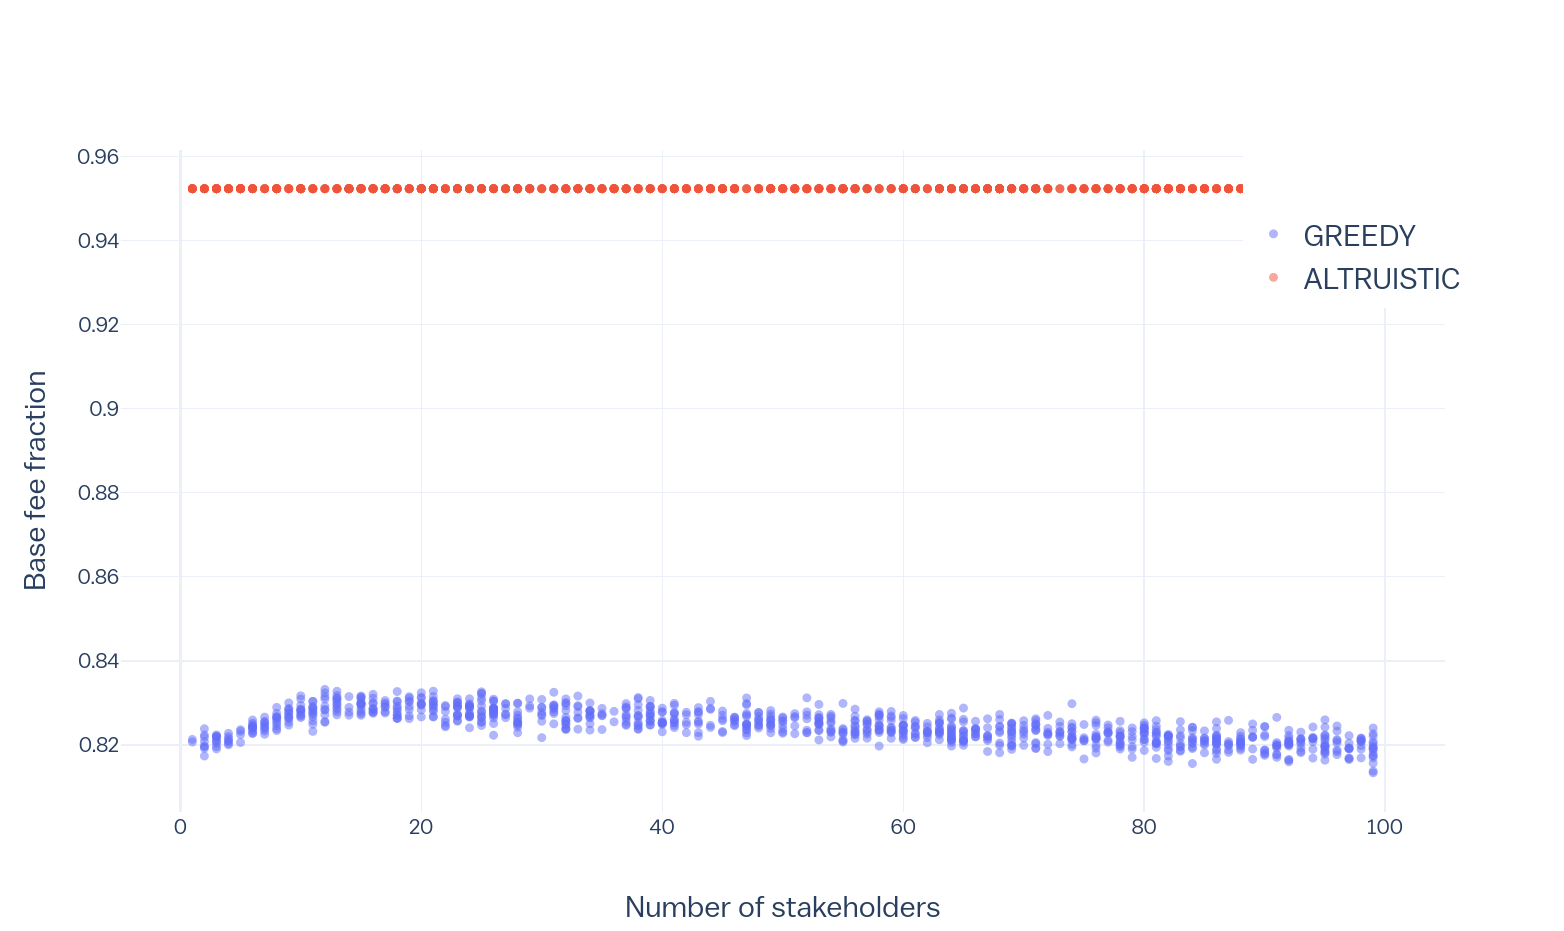
\includegraphics[width=0.8\linewidth]{standard-convergence.png}
    \caption{Base fee ratio for standard strategies}
    \label{standard-convergence}
\end{figure}

Figure \ref{standard-convergence} shows the \emph{base fee ratio}, or the fraction of fees paid as base fees rather than tips. A despot will keep this ratio close to 1, meaning that most fees are paid as base fees, since this gives the same revenue while reducing the number of times transactions have to be retried to be confirmed.

We see that \textsc{Altruistic} maintains an extremely high base fee ratio close to 1, since in this strategy proposers will not wait for higher tips before confirming transactions. \textsc{Greedy} still maintains a high ratio of around 0.82-0.84. Furthermore, this ratio is very collusion-insensitive --- it doesn't substantially change no matter how many stakeholders participate. Thus, even if all participants follow a short-sighted greedy algorithm for picking transactions, users can still use a simple bidding strategy of, say, bidding 30\% more than the base fee.

\begin{figure}[!h]
    \centering
    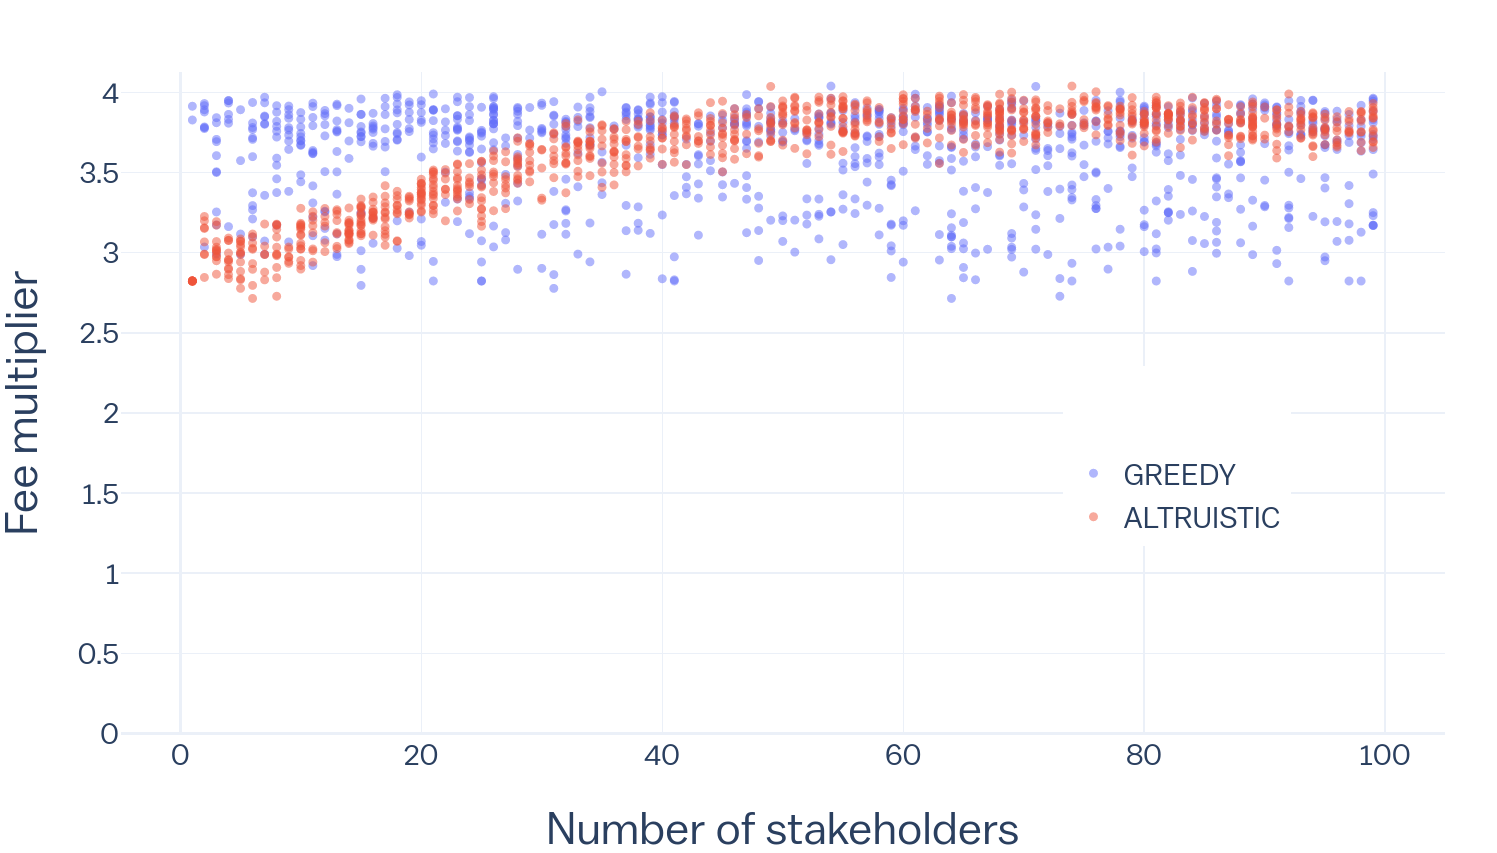
\includegraphics[width=0.9\linewidth]{standard-convergence-fees.png}
    \caption{Fee multiplier for standard strategies}
    \label{standard-convergence-fees}
\end{figure}

Figure \ref{standard-convergence-fees} shows the fee multiplier at the end of each simulation. We see that with both strategies, the fee multiplier ends up within a tight range --- the revenue-maximizing point. This is despite the fact that \textsc{HillClimb} is not very accurate at finding the revenue-maximizing point, especially when many stakeholders exist, due to its randomized nature.

\paragraph*{Greediness doesn't pay off} We now show that in a one-on-one contest, \textsc{Greedy} receives similar profits to \textsc{Altruistic}. We run a longer, 10000-block simulation, except this time we have one stakeholder following \textsc{Altruistic} and one stakeholder following \textsc{Greedy}.

\begin{figure}[!h]
    \centering
    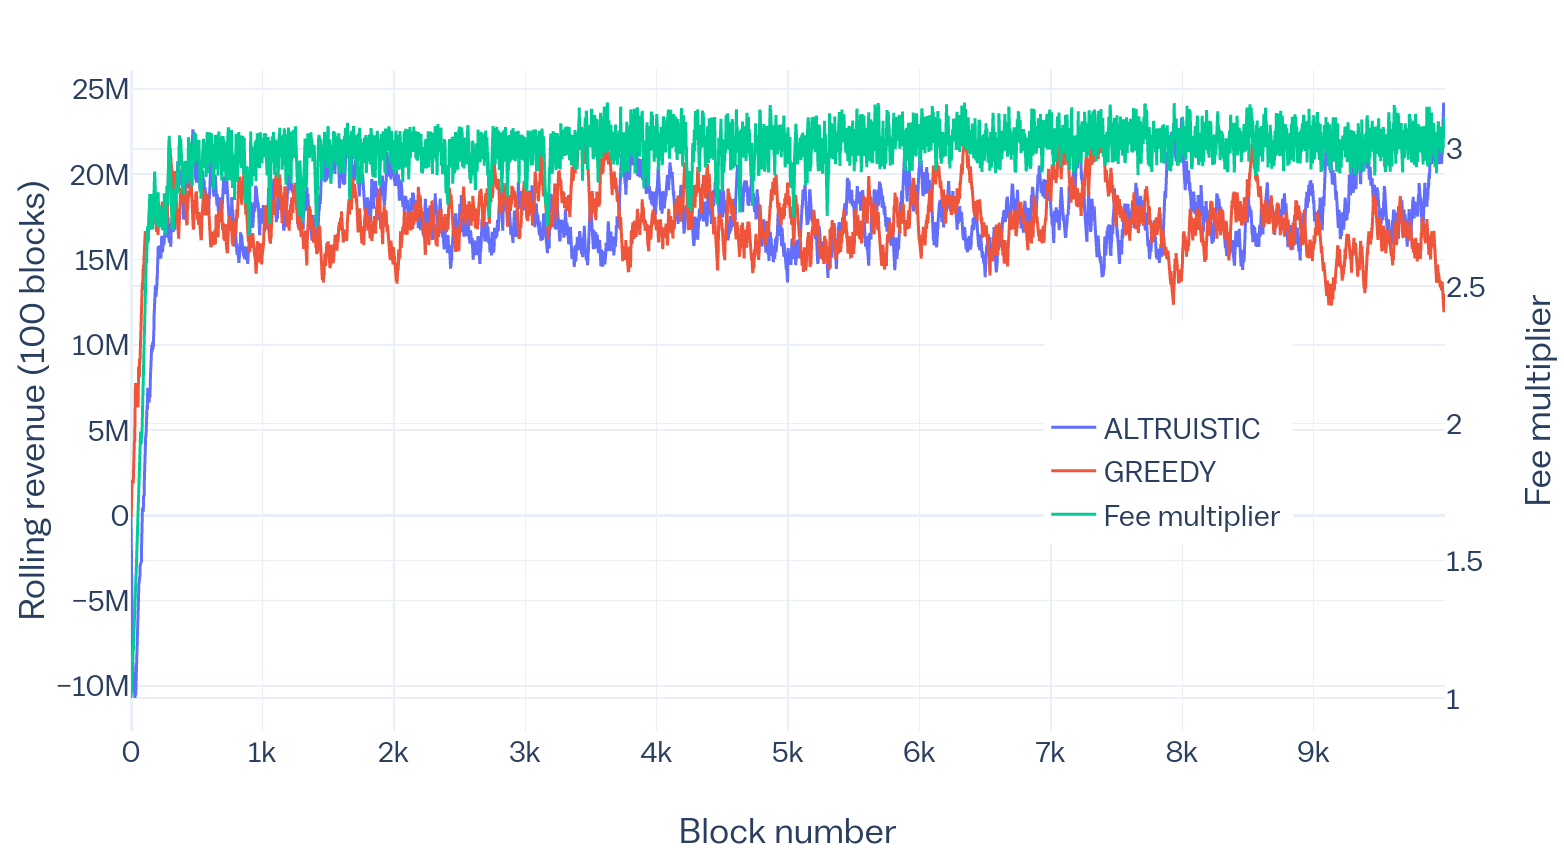
\includegraphics[width=0.9\linewidth]{no-greedy.png}
    \caption{Revenue for \textsc{Greedy} vs \textsc{Altruistic}}
    \label{no-greedy}
\end{figure}

We visualize a typical run of the simulation in Figure \ref{no-greedy}, which plots the revenue (averaged over 100 blocks) of both stakeholders, as well as the fee multiplier. We see that \textsc{Greedy} does not, in fact, gain more revenue than \textsc{Altruistic}. Intuitively, this is because when a \textsc{Greedy} proposer refuses to accept a transaction, and its tip is therefore forced upwards, the increased tip actually goes to the \emph{next} proposer, who may be following an \textsc{Altruistic} strategy. Thus, \textsc{Greedy}'s efforts to increase tips ends up being ``altruistic''.

\subsection{Pathological strategies}

We now look at the pathological strategies \textsc{Lazy} and \textsc{Monopolist}, showing that they always lose against standard strategies

\begin{figure}[!h]
    \centering
    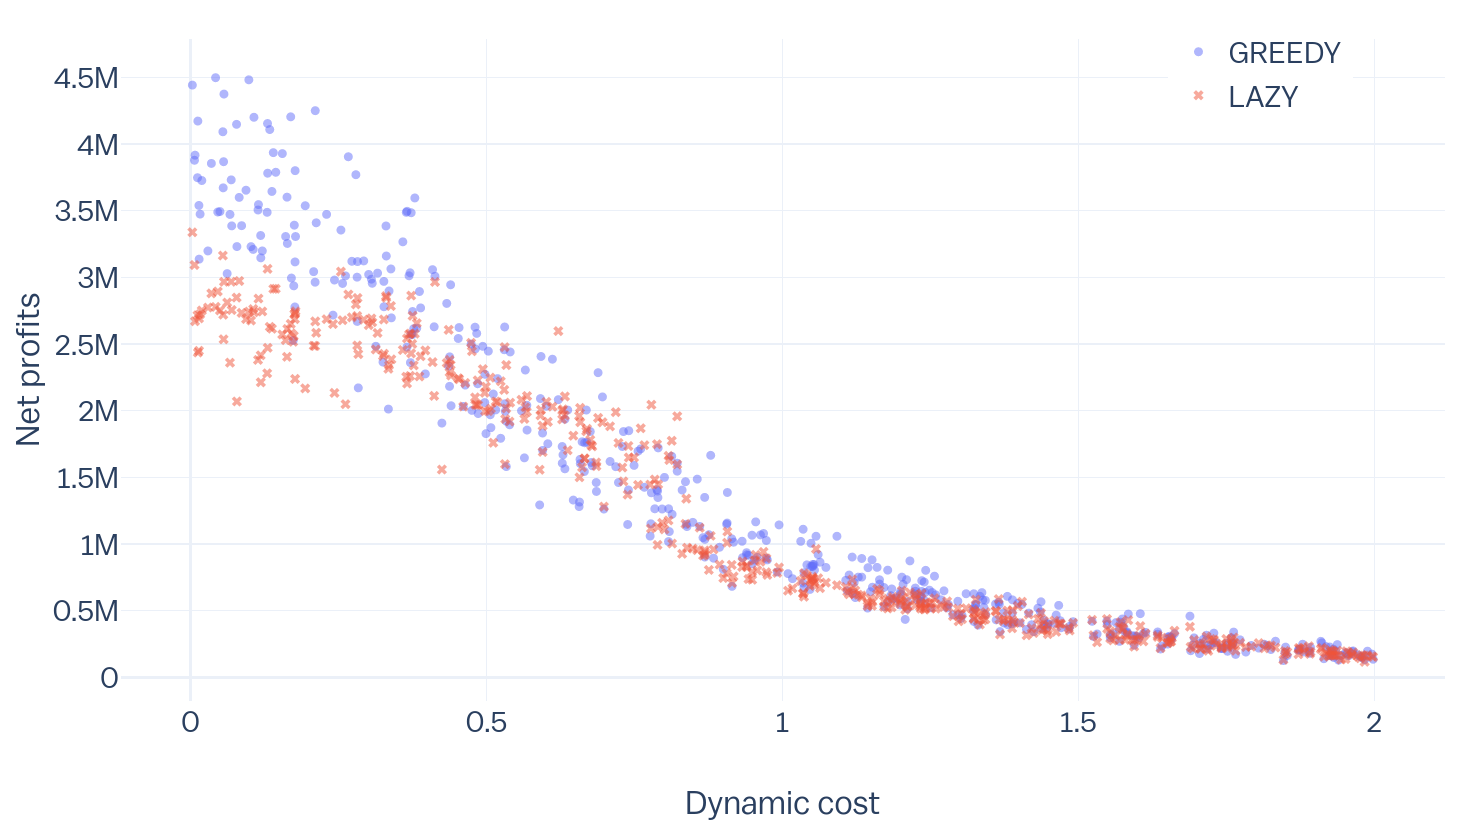
\includegraphics[width=0.8\linewidth]{greedy-vs-lazy.png}
    \caption{\textsc{Lazy} vs \textsc{Greedy}}
    \label{greedy-vs-lazy}
\end{figure}

\paragraph*{Laziness doesn't pay off} We first investigate the case where \textsc{Lazy} faces off head-to-head against \textsc{Greedy}. We run a 1000-block simulation, varying $S.\mathsf{dyncost}$ between 0 to 2 to represent differing opportunity costs for including a transaction. The results are shown in Figure \ref{greedy-vs-lazy} We see that at low costs, \textsc{Greedy} is much more profitable --- the profit gained by normally accepting transactions more than offset their costs. Even at higher costs, \textsc{Greedy} is still marginally better, since \textsc{Lazy} rejects even transactions that would have been profitable. Thus, a rational stakeholder would not choose \textsc{Greedy} as a strategy.

\paragraph*{Monopolists fail} We now investigate \textsc{Monopolist}, a strategy that picks all transactions, hoping to deny others revenue. We run a simulation analagous to our previous simulation, and plot the results in \ref{greedy-vs-mono}. We see that \textsc{Monopolist} is a strategy that's just as bad. At lower costs, it's basically equivalent to \textsc{Greedy}, since most transactions pay more fees than their cost. At higher costs, all \textsc{Monopolist} accomplishes is to waste money confirming transactions that pay low fees. Furthermore, comparing with Fig \ref{greedy-vs-lazy}, we see that \textsc{Monopolist} doesn't accomplish the goal of reducing \textsc{Greedy}'s revenue at any cost.

\begin{figure}[!h]
    \centering
    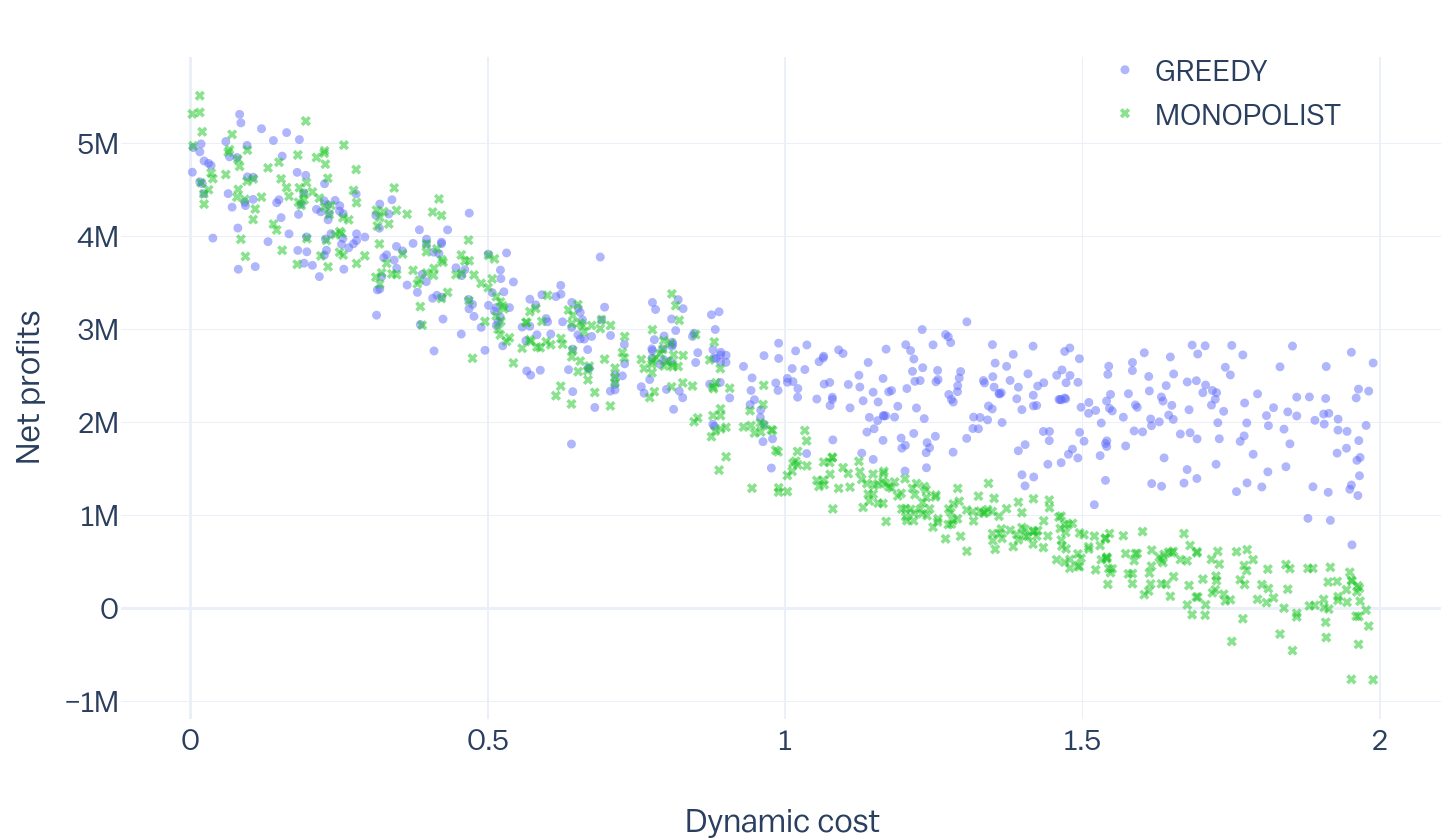
\includegraphics[width=0.8\linewidth]{greedy-vs-mono.png}
    \caption{\textsc{Monopolist} vs \textsc{Greedy}}
    \label{greedy-vs-mono}
\end{figure}

\subsection{Failure of alternative fee models}

Finally, we show that Synkletos's ``cartelizing'' feature of collectively setting a base fee that is then split is crucial to stability, despite it appearing to be unfair and monopolistic. To do so, we compare our model of Synkletos to an alternative model where instead of accumulating in the pool, fees are burned. This results in a system very similar to Ethereum's proposed EIP-1559 fee economy \cite{eip1559}.

We repeatedly run a 1000-block simulation with different numbers of \textsc{Greedy} stakeholders, comparing the outcome of EIP-1559's fee economy with that of Synkletos. Results are plotted in Figure \ref{eip}. We see that unlike Synkletos, which produces a stable fee multiplier regardless of the number of stakeholders, EIP-1559 suffers from two instabilities. First, at very low numbers of stakeholders (i.e. high levels of collusion), it's no longer in anyone's interest to correctly vote for the fee multiplier. Instead, everyone benefits from a low fee mulitplier that causes most fees to turn into tips. Secondly, at very high numbers \textsc{HillClimb} no longer converges, since the lack of a fee pool means revenue for stakeholders is extremely noisy. Most importantly, we see that Synkletos does not charge significantly more fees than EIP-1559.

\begin{figure}[!h]
    \centering
    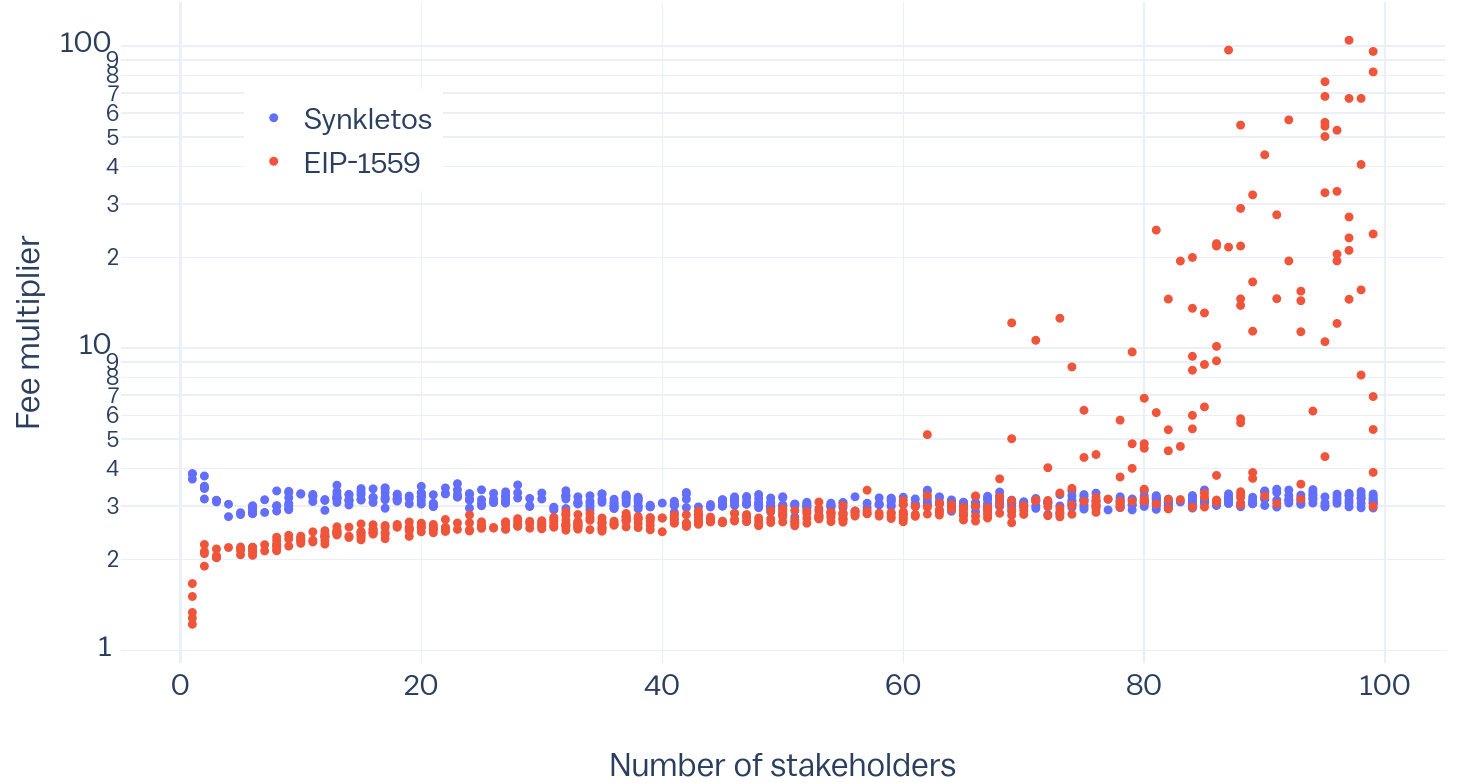
\includegraphics[width=0.8\linewidth]{eip.png}
    \caption{EIP-1995 vs Synkletos}
    \label{eip}
\end{figure}

\section{Conclusion}

In this chapter we described Synkletos, the cryptoeconomic system behind consensus in Themelio's. We first argued that instead of aiming for some sort of ideal outcome and trying to design a cryptoeconomic mechanism with just the right incentives to produce that outcome, we should aim for ``despot simulation'' --- having the blockchain function as if controlled by a rational, profit-seeking centralized entity. This allows us to design a mechanism that, unlike existing blockchain consensus mechanisms, is extremely resistant to collusion and provides for a much more user-friendly fee market.

We then validate our results by a stochastic agent-base simulation, showing that Synkletos reliably simulates a despot at varying levels of collusion, while resisting adversarial strategies. We also see that non-despot-simulating strategies like EIP-1559 do not produce stable behavior and can fail catastrophically when stakeholders collude.
\end{document}